\section{Further Fake Rate Discussion}
\label{sec:frFAQ}

Here we address some general questions about the 
Fake Rate (FR) method that have been asked in many 
different occasions.  They are
\begin{enumerate}

\item What about the heavy flavor (HF) composition?  How can you
use the same method in this analysis (where the fakes are mostly
not from HF) and in the untagged analysis (where the fakes are 
mostly from HF)?

\item What is this story of the parton $P_T$ dependence all
about?

\item Why do you take 50\% as an uncertainty?

\item If you have an over-prediction in the $t\bar{t}$ 
closure test, why don't you correct for that?

\item Can this be improved?

\end{enumerate}

\subsection{Heavy Flavor composition}
\label{sec:HF}

The first thing to realize is that this question only really 
applies to electrons.  Reasonably high $P_T$
muons in CMS that are not from EWK sources
are dominantly from HF, e.g.,

\begin{itemize}

\item Typically we find that 85-90\% of Fakeable Objects (FO) 
in the QCD MC are from HF. 

\item Even for this analysis, where the HF lepton background
in $t\bar{t}$ has been strongly suppressed by the 
$\geq 2$ btag requirement,
the remaining muon BG is mostly from HF.
This can be best seen by the entries corresponding to the 
lines $t\overline{t}\rightarrow \ell(b\rightarrow \ell)X$
and $t\overline{t}\rightarrow \ell(\slashed{b}\rightarrow \ell)X$
in the $\mu\mu$ column of Table~\ref{tab:yield_baseline}.
This shows that in $t\bar{t}$ MC the predicted BG with 
muons from HF ($\approx$ 0.14 events) is much larger than the 
BG with muons from other sources ($\approx$ 0.02 events).

\end{itemize}

For electrons, the HF dependence can be controlled by
carefully choosing what to use in the ``extrapolation'', {\it i.e.},
what electron requirements are loosened in going from the full
electron selection to the FO selection.  This is discussed in
Reference~\cite{frmethod}.  Briefly, there are three general
ways of defining the FO (V1, V2, V3):

\begin{itemize}
\item    V1 = extrapolate in ID and ISO
\item   V2 = extrapolate in ID only
\item   V3 = extrapolate in ISO only 
\end{itemize}

Extrapolating in ID introduces a HF dependence:
electrons in HF are ``real'', therefore the extrapolation in
ID depends on the HF composition.
If one does not worry about HF, V1 and V2 are sensible
choices, with some distinct advantages over V3, namely:
V2 is the most stable wrt parent parton $P_T$ and
V1 gives the best statistical power.
In the $H \to WW$ analysis, for example, we use V1.
On the other hand, V3 is the most stable against the HF dependence,
but has the worst parton $P_T$ dependence (this dependence
will be discussed in Section~\ref{sec:frpartonpt}).

For SUSY analyses we worry about HF and we use V3, {\it i.e.},
we extrapolate mostly in ISO.
A priori we do not expect a huge dependence of V3 on HF
because the FR of fake electrons from udsg and
HF cannot be that different: in both cases we are 
talking about electrons originating from jets, and the 
properties of jets from udgs are not markedly different 
from those from b.  But this needs to be tested, see below.

We have performed these tests a few times, the best record
of these is Reference~\cite{frmethod}.  Here we summarize 
the results from that note.

We measure the electron FR in data QCD events with an away jet of
40 GeV.  We then apply this FR to FO in QCD events selected 
in the same way but with the away jet b-tagged. We compare
the yield predicted by the FR method 
with the number of electrons passing the cuts in the sample. 
We find a ratio predicted/observed = $1.17 \pm 0.05$.
Note that this test is not 100\% clean.
There is an additional bias because the act
of tagging most likely changes the underlying $P_T$ of the
partons in the event (for example: btagging is not flat vs
jet $P_T$).  

We also perform the same test in MC.  Here we did not have enough stats,
so we had to use the muon-enriched sample. This 
may introduce
yet more bias on the away jet (now the away jet not only
is b-tagged, but it is most likely a $b \to \mu$ decay).
The result on MC is predicted/observed = $0.75 \pm 0.06$.

The bottom line is that we find that enriching the sample in HF changes the 
electron FR by something of order 20\%.  These changes
are due to some combination of HF effects and kinematical
changes in the sample due to the HF enrichment requirements.
We did not try to separate them out.  But the conclusion
is that the method works well enough on both HF-rich and
HF-poor event samples in both data and MC. 

It is also interesting to note that the V1 and V2 FR 
lead to an underprediction in the HF enriched samples,
just as can be argued from first principles.
For data we find  predicted/observed = $0.69 \pm 0.07$
and $0.60 \pm 0.06$ for V1 and V2 respectively; in MC we find 
predicted/observed = $0.27 \pm 0.04$ (V1) and
$0.30 \pm 0.04$ (V2).

Finally, just for fun, we repeat the exercise for muons.
In data we find predicted/observed = $1.03 \pm 0.03$, perfectly
consistent with 1; in MC we find 
this ratio to be $0.81 \pm 0.01$, suggesting that indeed 
there must be some bias in going from the QCD to the muon
enriched sample.

\subsection{Parton $P_T$ dependence}
\label{sec:frpartonpt}

The isolation of a lepton of a given $P_T$ depends 
on the $P_T$ of the mother parton.  This is easy 
to understand, {\em e.g.}, a 19 GeV muon from the
decay of a 20 GeV $b$-quark will be quite isolated
because the rest of the $b$-decay products can only
take up 1 GeV of momentum.  On the other hand a 19 GeV
muon from the decay of a 60 GeV $b$-quark will be much
less isolated.

\begin{figure}[htb]
\begin{center}
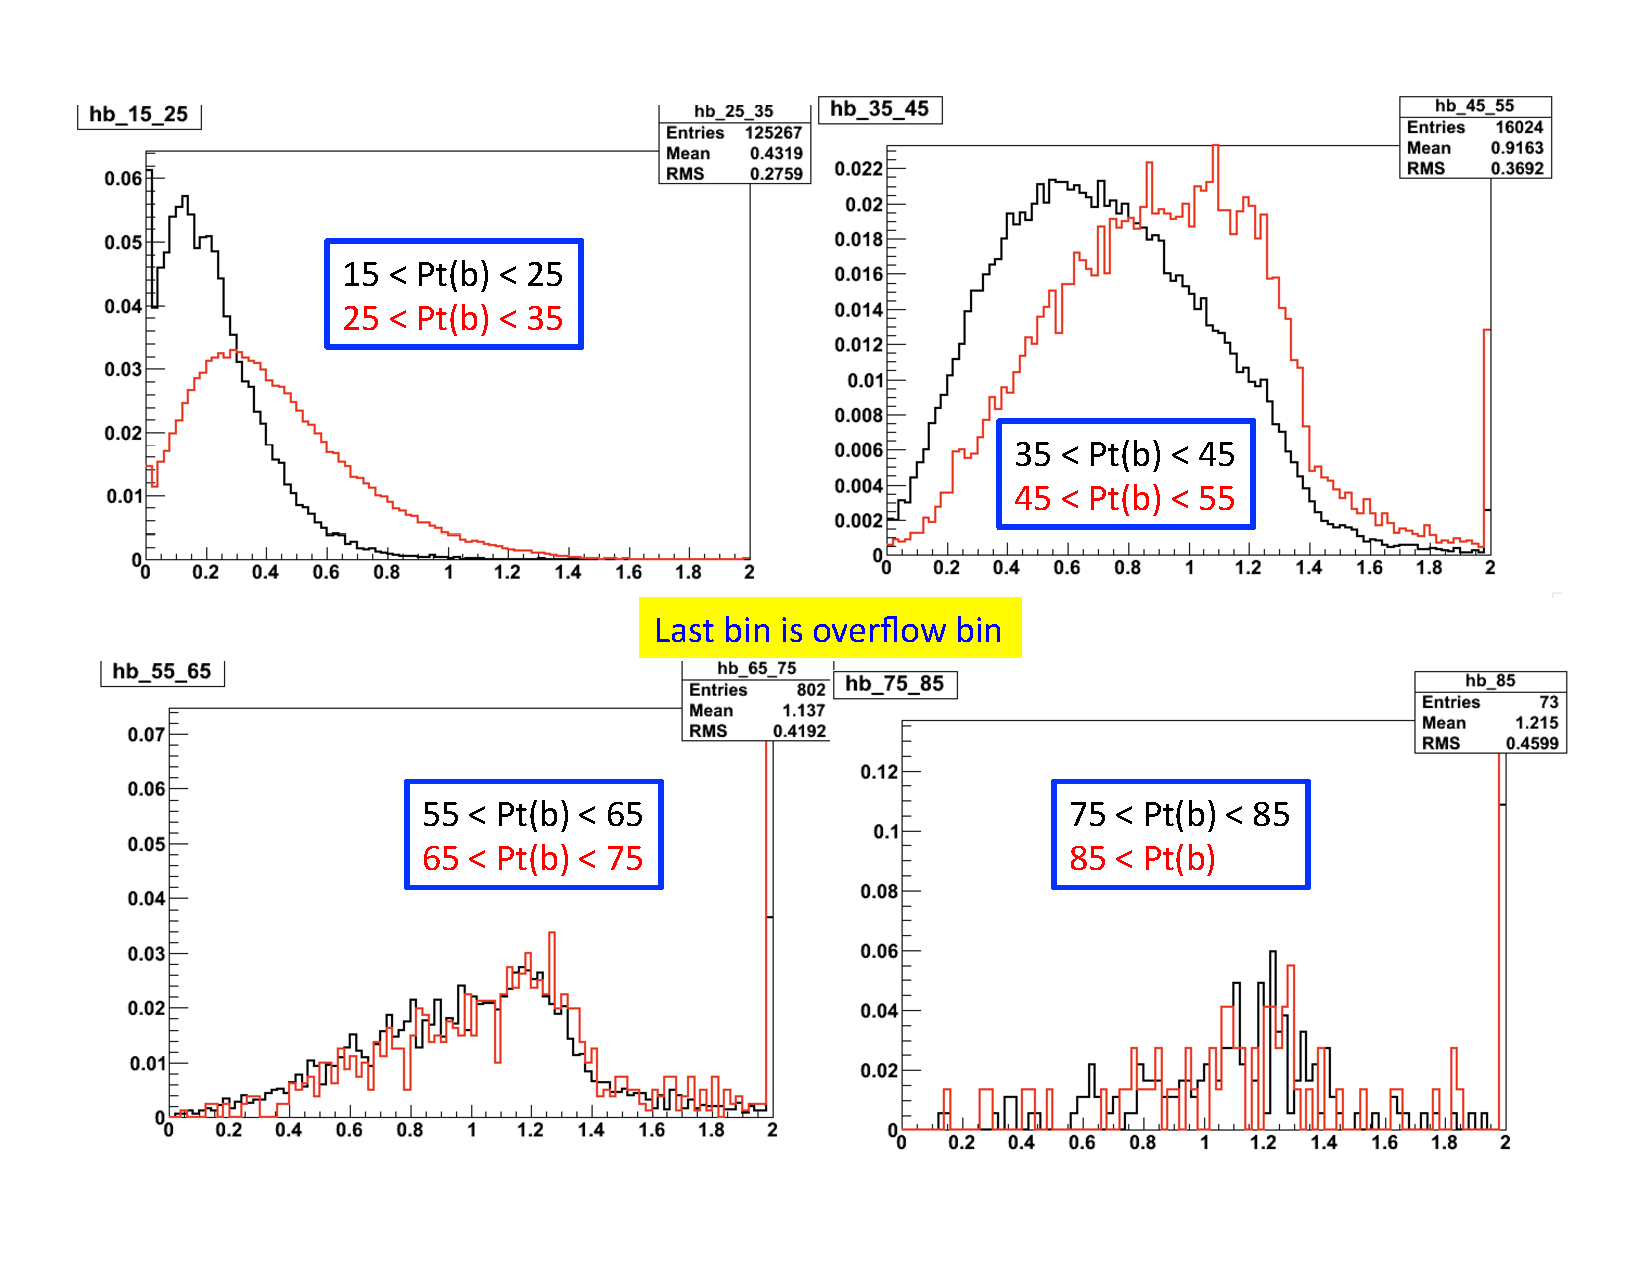
\includegraphics[width=0.75\linewidth]{figs/slavaIso.pdf}
\caption{Isolation for a MC muon from $b \to \mu$ decays
of 14 GeV $< P_T <$ 16 GeV for different intervals of the
parent $b$-quark $P_T$.
\label{fig:slavaIso}}
\end{center}
\end{figure}

This is a \textbf{huge} effect, as can be seen from 
Figure~\ref{fig:slavaIso}.  As a result, extrapolations
in isolation are very sensitive to the parent parton $P_T$
distribution.  We have found that this effect can be mitigated
by reducing the range of isolation over which we extrapolate.
This is why all our isolation extrapolations start from 
iso $<$ 0.4 or 0.6, not iso $< \infty$.

The muon FR is essentially an extrapolation in isolation
since it is almost\footnote{The other handle is 
impact parameter, which is used and 
which is insensitive to the parton $P_T$; however, by itself
it does not provide enough of a lever arm.}
the only handle that can be used
to separate fake muons from EWK muons.
Thus the muon FR, as well as the V3 electron FR, are quite
sensitive to the $P_T$ of the partons from which the 
lepton originates.


Figures~\ref{fig:frmuon} and~\ref{fig:frelectron} show
the muon and electron FR measured in data QCD events with 
different minimum requirements on the away jet $P_T$.  
To the extent that these events are mostly di-jets, 
the away jet $P_T$ is a measure of the $P_T$ of the 
parton from which the lepton originates.  We see that
as we reduce the away jet $P_T$ the FR goes up.
This is what is expected from Figure~\ref{fig:slavaIso}.

We think that it would be a mistake to take the variations
of Figures~\ref{fig:frmuon} and~\ref{fig:frelectron} too 
literally.  The away jet $P_T$ is only an approximation
to the parent parton $P_T$.  Things are not that simple.
For example, there are 3-jet events, there is gluon splitting
inside a jet, and last but not least the $P_T$ distributions
of jets in QCD events is steeply falling, while the $P_T$ 
distribution of jets in the backgrounds to dileptonic SUSY 
sources is not.  

\subsection{Where does the 50\% uncertainty come from?}
\label{sec:FRunc}

Most (all?) systematic uncertainties are judgement calls.
The choice of 50\% (over)covers the variations of 
Figures~\ref{fig:frmuon} and~\ref{fig:frelectron}. It 
(over)covers the variations seen in the HF tests 
(Section~\ref{sec:HF}). It just-about covers the 
closure tests in the $t\bar{t}$ sample (Table~\ref{tab:ttclosure}
in this note, but also results from References~\cite{ssnote2011}
and~\cite{frmethod}).
After playing around with various
options, and after having looked under the hood as we were developing
this methodology as far back as 2008, we have developed a sense
of how much we can trust the method.  It is not perfect:
50\% is perhaps conservative but we feel is a  
realistic estimate.  Finally, 50\% is a nice round number.

\subsection{Why not correct for the over prediction in $t\bar{t}$ MC?}
\label{sec:frcorrect}

We are not correcting for the overprediction in $t\bar{t}$ MC
(Table~\ref{tab:ttclosure}) for the following reasons.

In a search for new physics we prefer to err on the side of 
overestimating rather than underestimating the background.  The 
resulting ``overoptimism'' of the limits is not a big effect, 
see Table~\ref{tab:outreach}.

We do not fully understand where this overprediction 
comes from, and so we are not comfortable correcting for it.  
The hypothesis is that it is due to differences
in parton $P_T$ between $t\bar{t}$ and the QCD sample where
the FR is measured.  We have evidence that there is
an effect of this sort,
see Section 11.3 and Figure 7 of Reference~\cite{frmethod},
but it was not quantified at the time.  Since then we have 
tried to look at this in more detail. Preliminary results
point in the same direction, but the studies were never completed.

Finally, in the limit that the data and MC QCD FR are the same, the 
correction is equivalent to counting FO in data and 
multiplying them by the ratio of BG leptons to FO in MC.
This seems to us to be going a bit too far away from 
the data driven methodology.  

\subsection{Can the method be improved?}
\label{sec:frimprove}

The method can be improved by reducing the parton $P_T$ dependence
of the FR.  One would need to ``sculpt'' the away-jet $P_T$ 
distribution to better match the expected $P_T$ distribution
of partons in the BG.  This assumes that we can indeed show 
quantitatively that the overprediction in $t\bar{t}$ is from
parton $P_T$.

One of these days, when we are not in a mad rush for ICHEP or Moriond,
or chasing some SUSY scan, or fixing the hyphens in the 
paper drafts, or adding lines of NLL+NLO+PDF uncertainties
to cross-sections of processes that do not exist,
we might actually do it.  However we don't think
that we can go much below something like 30\% on the systematic 
uncertainty, and the improvement will not be a game changer.







